\section{Experimentación con shards}

\par Realizamos unas pruebas sobre la base de datos generada para ver el comportamiento y evaluar la performance de la misma ante un fuerte crecimiento.
Para esto generamos 3 shards en los cuales almacenamos la tabla \textit{clientes}. Luego fuimos insertando datos y cada cierta cantidad realizamos una serie de consultas y medimos el tiempo de respuesta:
\begin{itemize}
  \item Obtener una fila: por medio de un id hacemos un \textit{find} de una fila.
  \item Obtener 50 filas: utilizando un rango de valores del campo \textit{dni} (valor único) para filtrar un \textit{find0}.
  \item Obtener todas las filas: hacemos un \textit{find} sin restricciones.
\end{itemize}

\par Comenzamos sin ninguna fila en la base de datos y llegamos a una cantidad de 520000 filas aproximadamente.
Los resultados pueden observarse en la figura \ref{fig:testing}.

\begin{figure}
  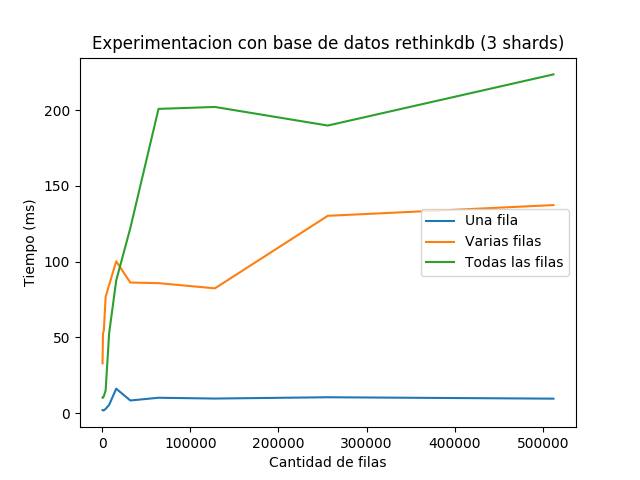
\includegraphics[width=\textwidth]{src/shards-testing.png}
  \caption{Experimentación de performance de shards al aumentar el tamaño de la base de datos.}
  \label{fig:testing}
\end{figure}

\par En principio no creíamos tener tan buena respuesta, o al menos notar una diferencia mas notoria superando los 200000.
Pero como vemos en el gráfico el tiempo de respuesta para obtener una fila es bastante estable, y los tiempos para obtener un grupo de filas o todas las filas no aumenta de forma tan fuerte (mas bien es lineal).

\par El tiempo de inserción no fue mucho, pero al insertar tanta cantidad el tiempo de corrida del script se hizo largo (alrededor de 4 horas).
